\chapter{Mechanical problem} \label{ch:mechanical_problem}

In the following chapter, the general framework presented in the previous chapter is applied to a purely mechanical analysis, neglecting the thermal terms.

\subsection{Mechanical constitutive initial value problem}

In the purely mechanical case, with all the quantities related to the thermal domain removed, a constitutive model based on internal variables is established by the following set of equations
    \begin{gather}
        \mat P = \rho_0 \frac{\partial \psi}{\partial \mat F},\\
        \psi = \psi(\mat F,\mat \alpha),\\
        \dot{\vect \alpha} = f(\mat F, \vect \alpha).
    \end{gather}
  Thus, the spatial mechanical constitutive initial value problem can be stated as follows
  \begin{problem}[Spatial mechanical constitutive initial value problem.]
  GGiven the initial values of the internal variables, $\vect \alpha(t_0)$, and the history of the deformation gradient
  \begin{equation}
      \mat F(t),\quad t\in[t_0,t_\text{end}],
  \end{equation}
  find the functions for $\mat \sigma(t)$ and $\vect \alpha(t)$ such that the constitutive equations
  \begin{gather}
      \mat \sigma = \rho \frac{\partial \psi}{\partial \mat F} \mat F^T,\\
      \psi = \psi(\mat F, \vect \alpha),\\
      \dot{\vect \alpha} = f(\mat F, \vect \alpha).
  \end{gather}
  are satisfied for every $t\in [t_0, t_\text{end}]$.
  \end{problem}

Likewise, in a material description it can be stated as
    \begin{problem}[Material mechanical constitutive intial value problem.]
    GGiven the initial values of the internal variables, $\vect \alpha(t_0)$, and the history of the deformation gradient
    \begin{equation}
        \mat F(t),\quad t\in[t_0,t_\text{end}],
    \end{equation}
    find the functions for $\mat P(t)$ and $\vect \alpha(t)$ such that the constitutive equations
    \begin{gather}
        \mat P = \rho_0 \frac{\partial \psi}{\partial \mat F},\\
        \psi = \psi(\mat F, \vect \alpha),\\
        \dot{\vect \alpha} = f(\mat F, \vect \alpha).
    \end{gather}
    are satisfied for every $t\in [t_0, t_\text{end}]$.
    \end{problem}

\subsection{Weak equilibrium. The principle of virtual work}

The strong equations that enforce the equilirium of a body can be writen using the spatial description as
\begin{equation}
  \rho \ddot{\bm u} = \operatorname{div}\bm \sigma + \bm b\quad \text{in $\Omega$},
\end{equation}
and the material description as
\begin{equation}
  \rho_0\ddot{\bm u} = \operatorname{div}_0 \bm P + \bm b_0\quad \text{in $\Omega_0$}.
\end{equation}
From a practical standpoint, finding the exact solution to the strong equilibrium equations in the context of real engineering problems is most often nearly or entirely impossible.
Most numerical methods obtain only approximate solutions to the so-called weak equilibrium equations to circumvent this problem.
These result from relaxing the strong equilibrium equations so that the solutions need only satisfy the equilibrium equations in an average sense instead of satisfying them pointwise.
This is achieved through an integration over the body volume.
The weak equilibrium equations can be found making use of several energetic and weighted residual methods, such as the Virtual Work Principle used here.
\enlargethispage{\baselineskip}
\begin{problem}[Principle of virtual work (spatial version).]
TThe Virtual Work Principle states, in a spatial description, that the body is in equilibrium if and only if the Cauchy stress field satisfies
    \begin{equation}
        \int_\Omega [\mat \sigma:\nabla \vect \eta - (\vect b -\rho \ddot{\bm u})\cdot \vect \eta]\ud v - \int_{\partial\Omega} \vect t\cdot \vect \eta\ud a = 0,\quad \forall \vect \eta \in \mathscr{V}_u,
    \end{equation}
 where $\mathscr{V}_u$ is the space of virtual displacement of the body, defined by the space of sufficiently regular arbitrary displacements
 \begin{equation}
     \vect \eta\colon \Omega\to  \mathscr{U}
 \end{equation}
 where $\mathscr{U}$ is the $n$-dimension vector associated with $\mathscr{E}$.
 \end{problem}


The principle of virtual work can be expressed in a completly equivalent way using a material description.
\begin{problem}[Principle of virtual work (material version).]
TThe Virtual Work Principle states, in a material description, that the body is in equilibrium if and only if the First Piola-Kirchhoff stress field satisfies
    \begin{equation}
        \int_{\Omega_0} [\mat P:\nabla_0 \vect \eta - (\vect b_0 - \rho_0 \ddot{\bm u})\cdot \vect \eta]\ud v - \int_{\partial\Omega_0} \vect t_0\cdot \vect \eta\ud da = 0,\quad \forall \vect \eta \in \mathscr{V}_{u,0},
    \end{equation}
 where $\mathscr{V}_{u,0}$ is the space of virtual displacement of the body, defined by the space of sufficiently regular arbitrary displacements
 \begin{equation}
     \vect \eta\colon \Omega_0\to \mathscr{U}.
 \end{equation}
\end{problem}

\subsection{Mechanical constitutive initial boundary value problem} \label{sec:mechanical_constitutive_problem}

It is now possible to pose the mechanical constitutive initial value problem in its weak form.
Assume that a body $\mathscr{B}$ is made from a generic material, characterized by a given constitutive model, whose internal variables are known at the initial time, as presented in Figure \ref{fig:quasi_static_prob }.
In addition, it is assumed that the interior of the body was subjected to a prescribed history of body forces, $\vect b(\bm X, t)$, $t\in[t_0, t_\text{end}]$, and to the following boundary conditions:
\begin{itemize}
    \item \textbf{Natural (or Neumann) boundary condition:}
    The boundary portion $\Omega_\text{traction, 0}$ of $\mathscr{B}$ is subjected to a prescribed history of traction forces, $\vect t_\text{presc}(\vect X, t)$, $\vect X\in \partial \Omega_\text{traction,0}$, $t\in[t_0, t_\text{end}]$,\\
    \item \textbf{Essential (or Dirichlet) boundary condition:}
    The boundary portion $\Omega_\text{motion, 0}$ of $\mathscr{B}$ is subjected to a prescribed displacement field history, $\vect u_\text{presc}(\vect X, t)$, such that $$\vect \varphi(\vect X, t) = \vect X + \vect u_\text{presc}(\vect X, t),\quad \vect X\in \partial\Omega_\text{motion, 0},\quad t\in[t_0, t_\text{end}].$$
\end{itemize}

\begin{figure}
  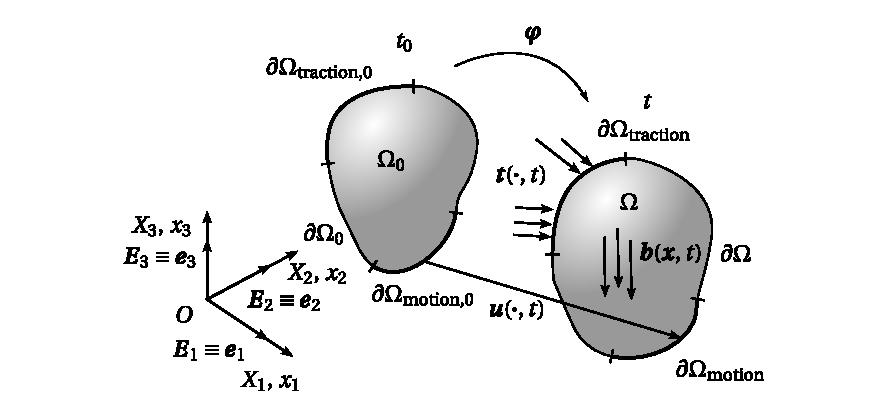
\includegraphics[width=.9\textwidth]{quasi_static_prob}
  \caption{Quasi-static mechanical constitutive initial boundary value problem.}
\label{fig:quasi_static_prob}
\end{figure}

It is also convenient to define the set of kinematically admissible displacements of $\mathscr{B}$ as the set of all sufficiently regular displacement functions tha satisfy the essential boundary condition \citep{de_souza_neto_computational_2008},
\begin{highlight}[innertopmargin=-5pt]
    \begin{multline}
        \mathscr{K}_u\equiv \{\vect u:\Omega_0\times \mathscr{R}\to \mathscr{U}\;|\;\vect u(\vect X,t) = \vect u_\text{presc} (\vect X,t),\\ \vect X\in\partial \Omega_\text{motion,0},\quad t\in [t_0,t_\text{end}]\}.\quad
    \end{multline}
\end{highlight}

So the weak form of the quasi-static mechanical constitutive initial boundary value problem can be stated in a spatial description as follows
\begin{problem}[Spatial mechanical initial BVP.]
    FFind a kinematically admissible displacement function, $\vect u\in \mathscr{K}_u$, such that for every $t\in [t_0,t_\text{end}]$, the body $\mathscr{B}$ is in equilibrium as stated by the Virtual Work Principle
        \begin{equation}
        \int_\Omega [\mat \sigma:\nabla \vect \eta - (\vect b-\rho\ddot{\bm u})\cdot \vect \eta]\ud v - \int_{\partial\Omega} \vect t\cdot \vect \eta\ud a = 0,\quad \forall \vect \eta \in \mathscr{V}_u,
    \end{equation}
    where the space of virtual displacements at time $t$ is defined by
    \begin{equation}
        \mathscr{V}_u \equiv \left\{\vect \eta:\Omega\to \mathscr{U}\;|\;\vect \eta = \vect 0\quad \text{in}\quad \bm \varphi(\partial\Omega_\text{motion,0},t)\right\},
    \end{equation}
    and at each point of $\mathscr{B}$, the Cauchy stress tensor is the solution of spatial mechanical constitutive initial values problem.
\end{problem}
and in the material description as
\begin{problem}[Material mechanical initial BVP.]
    FFind a kinematically admissible displacement function, $\vect u\in \mathscr{K}_u$, such that for every $t\in [t_0,t_\text{end}]$, the body $\mathscr{B}$ is in equilibrium as stated by the Virtual Work Principle
        \begin{equation}
        \int_{\Omega_0} [\mat P:\nabla_0 \vect \eta - (\vect b_0-\rho_0\ddot{\bm u})\cdot \vect \eta]\ud v - \int_{\partial\Omega_0} \vect t_0\cdot \vect \eta\ud a = 0,\quad \forall \vect \eta \in \mathscr{V}_{u,0},
    \end{equation}
    where the space of virtual displacements at time $t$ is defined by
    \begin{equation}
        \mathscr{V}_{u,0} \equiv \left\{\vect \eta:\Omega_0\to \mathscr{U}\;|\;\vect \eta = \vect 0\quad \text{in}\quad \partial\Omega_\text{motion,0}\right\},
    \end{equation}
    and at each point of $\mathscr{B}$, the First Piola-Kirchhoff stress tensor is the solution of material mechanical constitutive initial values problem.
\end{problem}

\section{Time discretization for the constitutive equations} \label{sec:time_discretization}

Given a generic path-dependent model, i.e., a model in which the stress state does not depend only on the instantaneous deformation state but also on the deformation history, the solution of the constitutive initial value problem for a given set of initial conditions is usually not known for complex strain paths $\mat F(t)$.
Thus, there is a need to use an appropriate numerical algorithm to integrate the rate constitutive equations.

In general, the algorithms for integrating rate constitutive equations are obtained adopting some time (or pseudo-time) discretization and some hypothesis on the deformation path between adjacent time stations.
In the present document, an algorithm is adopted based on approximated incremental constitutive functions.
Attending to the mechanical constitutive initial boundary value problem and considering the time increment $[t_n, t_{n+1}]$, this approach is comprised by the following two requirements:
\begin{itemize}
    \item \textbf{Cauchy and First Piola-Kirchhoff stress tensors.}   Considering a time increment $[t_n, t_{n+1}]$ and given the set $\vect \alpha_n$ of internal variables at $t_n$, the deformation gradient $\mat F_{n+1}$ at time $t_{n+1}$ determines the stress $\mat \sigma_{n+1}$ uniquely through
    \begin{highlight}
        \begin{equation}
            \mat \sigma_{n+1} = \hat{\mat \sigma}(\vect \alpha_n, \mat F_{n+1}), \label{eq:incremental_stress}
        \end{equation}
    \end{highlight}
    where $\hat{\vect \sigma}$ is the incremental constitutive function for the Cauchy stress tensor.

    Similarly, the First Piola-Kirchhoff stress tensor $\mat P_{n+1}$ must be uniquely determined by the prescribed deformation gradient $\mat F_{n+1}$ prescribed at $t_{n+1}$ as
    \begin{equation}
        \mat P_{n+1} = \hat{\mat P}(\mat \alpha_n, \mat F_{n+1}),
    \end{equation}
    where $\hat{\mat P}$ is the incremental constitutive function for the First Piola-Kirchhoff stress tensor.
    \item \textbf{Set of internal variables.} Assuming that the set of internal variables $\vect \alpha_n$ is known at $t_n$, the set of internal variables must be uniquely determined by the prescribed deformationgradient $\mat F_{n+1}$ prescribed at $t_{n+1}$ as
    \begin{highlight}
        \begin{equation}
             \vect \alpha_{n+1} =\hat{\vect \alpha}(\vect \alpha_n, \mat F_{n+1}), \label{eq:incremental_flux}
        \end{equation}
    \end{highlight}
    where $\hat{\vect \alpha}$ is the incremental constitutive function for the set of internal variables.
\end{itemize}

Generally, the numerical constitutive laws are nonlinear and path-independent within one increment.
In other words, within each increment, $\mat \sigma_{n+1}$ and $\vect \alpha_{n+1}$, they are functions of $\mat F_{n+1}$ alone with the argument $\vect \alpha_n$ constant within the same time interval.

Making use of the aforementioned time discretization, one can state the weak form of the mechanical constitutive initial boundary value problem in the spatial description as
\begin{problem}[Spatial incremental mechanical initial BVP.]
    GGiven the set of internal variables $\vect \alpha_n$ at $t_n$, the prescribed body and traction force fields $\vect b_{n+1}$ and $\vect t_{n+1}$ at $t_{n+1}$, and the prescribed deformating gradient $\mat F_{n+1}$ at $t_{n+1}$, find the kinematically admissible displacement field $\vect u_{n+1}\in\mathscr{K}_{u,n+1}$ such that the body $\mathscr{B}$ is in equilibrium as stated by the virtual Work Principle
            \begin{equation}
        \int_{\Omega_{n+1}} [\hat{\mat \sigma}(\mat F_{n+1}, \vect \alpha_n):\nabla \vect \eta - (\vect b_{n+1}-\rho\ddot{\bm u}_{n+1})\cdot \vect \eta]\ud v - \int_{\partial\Omega_{n+1}} \vect t_{n+1}\cdot \vect \eta\ud a = 0,\quad \forall \vect \eta \in \mathscr{V}_u,
    \end{equation}
    where the space of kinematically admissible displacement fields $\mathscr{K}_{n+1}$ is defined by
    \begin{equation}
            \mathscr{K}_{u,n+1}\equiv \{\vect u:\Omega_0\times \mathscr{R}\to \mathscr{U}\;|\;\vect u_{n+1}(\vect X) = \vect u_\text{presc,$n+1$}(\vect X),\;\vect X\in\partial \Omega_\text{motion,0}\}.
    \end{equation}
\end{problem}
and in the material description as
\begin{problem}[Material incremental mechanical initial BVP.]
    GGiven the set of internal variables $\vect \alpha_n$ at $t_n$, the prescribed body and traction force fields $\vect b_{0,n+1}$ and $\vect t_{0,n+1}$ at $t_{n+1}$, and the prescribed deformating gradient $\mat F_{n+1}$ at $t_{n+1}$, find the kinematically admissible displacement field $\vect u_{n+1}\in\mathscr{K}_{u,n+1}$ such that the body $\mathscr{B}$ is in equilibrium as stated by the virtual Work Principle
            \begin{equation}
        \int_{\Omega_0} [\hat{\mat P}(\mat F_{n+1}, \vect \alpha_n):\nabla_0 \vect \eta - (\vect b_{0,n+1}-\rho_0\ddot{\bm u}_{n+1})\cdot \vect \eta]\ud v - \int_{\partial\Omega_{0,n+1}} \vect t_{0,n+1}\cdot \vect \eta\ud a = 0,\quad \forall \vect \eta \in \mathscr{V}_{u,0},
    \end{equation}
    where the space of kinematically admissible displacement fields $\mathscr{K}_{n+1}$ is defined by
    \begin{equation}
            \mathscr{K}_{u,n+1}\equiv \{\vect u:\Omega_0\times \mathscr{R}\to \mathscr{U}\;|\;\vect u_{n+1}(\vect X) = \vect u_\text{presc,$n+1$}(\vect X),\;\vect X\in\partial \Omega_\text{motion,0}\}.
    \end{equation}
\end{problem}

\section{Finite Element Method} \label{sec:fem_mech}

With the incremental weak form of the mechanical constitutive initial boundary value problem now established, an approximated solution can be found using the Finite Element Method.

\subsection{Finite element concept}

The first in the Finite Element method is to discretize the continuum domain $\Omega$ in a finite set of $n_\text{elem}$ mutually exclusive subdomains called finite elements $\Omega^{(e)}$.
The discretized domain, $^h\Omega$, is therefore an approximation to the continuum domain expressed by
\begin{equation}
    \Omega \approx {}^h\Omega \equiv \bigcup_{e=1}^{n_\text{elem}}\Omega^{(e)}.
\end{equation}
The spaces of virtual displacements $\mathscr{V}_u$ and \(\mathscr V_{u,0}\) as well as the space of kinematically admissible displacement fields $\mathscr{K}_u$ are also discretized in the same way, with their discretized forms denoted by $^h\mathscr{V}_u$, \(^h\mathscr{V}_{u,0}\) and $^h\mathscr{K}_u$.

\subsection{Interpolation functions}

Let $e$ be a generic finite element with $n_\text{nodes}$ nodes, where each node $i$ of coordinates $\vect x^i$ is associated with an interpolation function $N_i^{(e)}$.
These interpolation functions are often called shape functions and perform the required filed interpolations inside the element domain $\Omega^{(e)}$.

Letting $a(\vect x)$ be a generic field defined over $\Omega^{(e)}$, its interpolation at any point $\vect x$ inside the element is defined by the element shape functions as
\begin{highlight}
    \begin{equation}
        a(\vect x) \approx {}^ha(\vect x) \equiv \sum_{i=1}^{n_\text{nodes}} a(\vect x_i) N_i^{(e)}(\vect x).
    \end{equation}
\end{highlight}
If instead $a(\vect x)$ is instead a generic field defined over the global domain $\Omega$, the interpolation of $a(\vect x)$ at any point $\vect x$ is defined by the global shape functions as
\begin{highlight}
    \begin{equation}
        a(\vect x) \approx {}^h a(\vect x) \equiv \sum_{i=1}^{n_\text{points}} a(\vect x_i) N_i^g(\vect x), \label{eq:interpol_global}
    \end{equation}
\end{highlight}
where $n_\text{points}$ is the total number of nodes of the finite element mesh.
The discretized spaces $^h \mathscr{V}_u$ and $^h\mathscr{K}_u$ can now be defined as
\begin{align}
    ^h \mathscr{K}_u&\equiv \Big\{\vphantom{|}^h\vect u(\vect x) = \sum_{i=1}^{n_\text{points}} \vect u(\vect x_i) N_i^g(\vect x)\;|\; \vect u(\vect x_i) = \vect u_\text{presc}(\vect x_i)\quad\text{if $\vect x_i\in \partial\Omega_\text{motion,0}$}  \Big\},\\
    ^h\mathscr{V}_u&\equiv \Big\{\vphantom{|}^h\vect \eta(\vect x) = \sum_{i=1}^{n_\text{points} } \vect \eta(\vect x_i) N_i^g(\vect x)\;|\;\vect \eta(\vect x_i)=\vect 0\quad\text{if $\vect x_i\in \partial\Omega_\text{motion,0}$}   \Big\}
\end{align}
Quantities defined on the reference configuration \(\Omega_0\) accepted a treatment entirely similar to the one described above, and thus is omitted.

\subsection{Interpolation matrix and discrete gradient operators}

The global shape functions can be conveniently assembled in the so-called global interpolation matrix as
\begin{equation}
    \mathbf N^g(\vect x) \equiv \left[\text{diag}[N_1^g(\vect x)]\; \text{diag}[N_2^g(\vect x)]\;\cdots\; \text{diag}[N_{n_\text{points}}^g(\vect x)]\right],
\end{equation}
where $\text{diag}[N_i^g]$ is a diagonal matriz $n_\text{dim} \times n_\text{dim}$
\begin{equation}
    \text{diag}[N_i^g(\vect x)]\equiv \left[
    \begin{array}{cccc}
         N_i^g & 0 & \cdots & 0  \\
         0     & N_i^g & \cdots & 0 \\
         \vdots & \vdots & \ddots & \vdots \\
         0 & 0 & \cdots & N_i^g
    \end{array}
    \right]
\end{equation}
where $n_\text{dim}$ is the number of degrees of freedom per node.

Defining the global vector of nodal displacements as
\begin{equation}
    \mathbf u = \Big[ u_1^1,\dots,u^1_{n_\text{dim}},\dots, u_1^{n_\text{points}},\dots,u^{n_\text{points}}_{n_\text{dim}}\Big]^T,
\end{equation}
the displacement field $\bm u(\vect x)$ defined over the global domain $\Omega$, can be found from Equation \eqref{eq:interpol_global} at any point $\vect x$ as
\begin{highlight}
    \begin{equation}
        ^h\vect u(\vect x) \equiv \mathbf N^g(\vect x)\mathbf u,\quad {}^h\vect u\in {}^h\mathscr{K}_u.
    \end{equation}
\end{highlight}

\subsection{Spatial discretization} \label{sec:spatial_discretization_mech}

Applying the aforementioned finite element discretization to the incremental mechanical constitutive initial boundary value problem, we can then write in the spatial description
\begin{highlight}
    \begin{equation}
        \int_{^h\Omega}\left[\hat{\mat \sigma}^T\mathbf B^g\vect \eta - (\mathbf b_{n+1} - \rho\ddot{\mathbf u}_{n+1}) \cdot \mathbf N^g \vect \eta \right]\ud v -\int_{\partial ^h\Omega_\text{traction}} \mathbf t_{n+1}\cdot \mathbf N^g\vect \eta \ud a = 0,\quad \forall \vect \eta \in {}^h\mathscr{V}_u,  \label{eq:forma_fraca_disc}
    \end{equation}
\end{highlight}
where $\mathbf B^g$ is the discrete symmetric global gradient operator, defined for a 2D problem in cartesian coordinates as
\begin{equation}
    \mathbf B^g\equiv \left[
    \begin{array}{ccccccc}
         \displaystyle{\frac{\partial N_1^g}{\partial x}} & 0 & \displaystyle{\frac{\partial N_2^g}{\partial x}} & 0 & \cdots &
         \displaystyle{\frac{\partial N_{n_\text{points}}^g}{\partial x}} & 0\\
         0 & \displaystyle{\frac{\partial N_1^g}{\partial y}} & 0 & \displaystyle{\frac{\partial N_2^g}{\partial y}} & \cdots &
         0 & \displaystyle{\frac{\partial N_{n_\text{points}}^g}{\partial y}}\\
         \displaystyle{\frac{\partial N_1^g}{\partial y}} & \displaystyle{\frac{\partial N_1^g}{\partial x}} & \displaystyle{\frac{\partial N_2^g}{\partial y}} & \displaystyle{\frac{\partial N_2^g}{\partial x}} & \cdots &
         \displaystyle{\frac{\partial N_{n_\text{points}}^g}{\partial y}} & \displaystyle{\frac{\partial N_{n_\text{points}}^g}{\partial x}}
    \end{array}
    \right].
\end{equation}

Equation \eqref{eq:forma_fraca_disc} can be rewritten as
\begin{multline}
    \left\{  \int_{^h\Omega}\left[{\mathbf B^g}^T \hat{\mat \sigma}(\vect \alpha_n, \vect F_{n+1})-{\mathbf N^g}^T\mathbf b_{n+1} +{\mathbf N^g}^T\rho\ddot{\mathbf u}_{n+1} \right]\ud v \right. \\ \left. -\int_{\partial ^h\Omega_\text{traction}} {\mathbf N^g}^T \mathbf t_{n+1}\ud a\right\}^T\;\vect \eta =0,\quad \forall \vect \eta \in ^h \mathscr{V}_u, \label{eq:eq_forças}
\end{multline}
and, since it must be satisfied for any $\vect \eta \in {}^h \mathscr{V}_u$, the incremental quasi-static discretized mechanical constitutive initial boundary value problem can thus be stated in the spatial description as
\begin{problem}[Spatial incremental discretized mechanical initial BVP.]
GGiven the set of internal variables $\vect \alpha_n$ at $t_n$, the prescribed body and traction force fields $\vect b_{n+1}$ and $\vect t_{n+1}$, and the prescribed deformation gradient $\mat F_{n+1}$ at $t_{n+1}$, find the kinematically admissible nodal displacement field $\vect u_{n+1}\in {^h\mathscr{K}_{u,n+1}}$ such that the body $\mathscr{B}$ is in equilibrium as stated by the Virtual Work Principle
\begin{equation}
    \mathbf M \ddot{\mathbf u}_{n+1} + \mathbf f^\text{\;int}(\mathbf u_{n+1})-\mathbf f^\text{\;ext}_{n+1}=\mathbf 0, \label{eq:equilibrium_spatial}
\end{equation}
where $\mathbf f^\text{int}$ e $\mathbf f^\text{ext}_{n+1}$ are the global vectors of internal and external forces defined as
\begin{align}
    \mathbf f^\text{\;int} &\equiv \int_{^h\Omega}{\mathbf B^g}^T \hat{\mat \sigma}(\mat F_{n+1}, \vect \alpha_n)\ud v,\\
    \mathbf f^\text{\;ext}_{n+1} &\equiv \int_{^h\Omega}{\mathbf N^g}^T \mathbf b_{n+1}\ud v + \int_{\partial^h\Omega_\text{traction}}{\mathbf N^g}^T \mathbf t_{n+1}\ud a,
\end{align}
and $\mathbf M$ is the mass matrix defined as
\begin{equation}
  \mathbf M = \int_{{}^h\Omega} \rho {\mathbf{N}^g}^T\mathbf{N}^g \ud v.
\end{equation}
\end{problem}
In a material description, Equation \eqref{eq:eq_forças} is written as
\begin{multline}
     \left\{  \int_{^h\Omega_0}\left[{\mathbf G^g}^T \hat{\mat P}(\vect \alpha_n, \vect F_{n+1})-{\mathbf N^g}^T \mathbf b_{0,n+1} + {\mathbf N^g}^T \rho_0\ddot{\mathbf u}_{n+1} \right]\ud v \right.\\ \left.   -\int_{\partial ^h\Omega_\text{traction,0}} {\mathbf N^g}^T \mathbf t_{0,n+1}\ud a\right\}^T\;\vect \eta =0,\quad \forall \vect \eta \in ^h \mathscr{V}_{u,0},
\end{multline}
where $\mathbf G^g$ is the discrete global gradient operator, defined for a 2D problem in cartesian coordinates as
\begin{equation}
    \mathbf G^g\equiv \left[
    \begin{array}{ccccccc}
         \displaystyle{\frac{\partial N_1^g}{\partial x}} & 0 & \displaystyle{\frac{\partial N_2^g}{\partial x}} & 0 & \cdots &
         \displaystyle{\frac{\partial N_{n_\text{points}}^g}{\partial x}} & 0\\
         0 & \displaystyle{\frac{\partial N_1^g}{\partial x}} & 0 & \displaystyle{\frac{\partial N_2^g}{\partial x}} & 0 & \cdots &
         \displaystyle{\frac{\partial N_{n_\text{points}}^g}{\partial x}}\\
         \displaystyle{\frac{\partial N_1^g}{\partial y}} & 0 & \displaystyle{\frac{\partial N_2^g}{\partial y}} & \cdots &
         0 & \displaystyle{\frac{\partial N_{n_\text{points}}^g}{\partial y}} & 0\\
         0 & \displaystyle{\frac{\partial N_1^g}{\partial y}} & 0 & \displaystyle{\frac{\partial N_2^g}{\partial y}} & \cdots &
         0 & \displaystyle{\frac{\partial N_{n_\text{points}}^g}{\partial y}}\\
    \end{array}
    \right],
\end{equation}
and, as for the spatial description, it must  be satisfied for any $\vect \eta \in {}^h\mathscr{V}_{u,0}$, the incremental quasi-static discretized mechanical constitutive initial boundary value problem can thus be stated in the material description as
\begin{problem}[Material incremental discretized mechanical initial BVP.]
GGiven the set of internal variables $\vect \alpha_n$ at $t_n$, the prescribed body and traction force fields $\vect b_{0,n+1}$ and $\vect t_{0,n+1}$, and the prescribed deformation gradient $\mat F_{n+1}$ at $t_{n+1}$, find the kinematically admissible nodal displacement field $\vect u_{n+1}\in {^h\mathscr{K}_{u,n+1}}$ such that the body $\mathscr{B}$ is in equilibrium as stated by the Virtual Work Principle
\begin{equation}
    \mathbf M \ddot{\mathbf u}_{n+1} +\mathbf f^\text{\;int}(\mathbf u_{n+1})-\mathbf f^\text{\;ext}_{n+1}=\mathbf 0, \label{eq:equilibrium_material}
\end{equation}
where $\mathbf f^\text{\;int}$ e $\mathbf f^\text{\;ext}_{n+1}$ are the global vectors of internal and external forces defined as
\begin{align}
    \mathbf f^\text{int} &\equiv \int_{^h\Omega_0}{\mathbf G^g}^T \hat{\mat P}(\mat F_{n+1}, \vect \alpha_n)\ud v,\\
    \mathbf f^\text{ext}_{n+1} &\equiv \int_{^h\Omega_0}{\mathbf N^g}^T \mathbf b_{0,n+1}\ud v + \int_{\partial^h\Omega_\text{traction,0}}{\mathbf N^g}^T \mathbf t_{0,n+1}\ud a.
\end{align}
and $\mathbf M$ is the mass matrix defined as
\begin{equation}
  \mathbf M = \int_{{}^h\Omega_0} \rho_0 {\mathbf{N}^g}^T\mathbf{N}^g \ud v.
\end{equation}
\end{problem}

The global vectors for the internal and external forces are usually obtained by assemblage of their elemental counterparts as
\begin{gather}
    \mathbf f^\text{\;int} = \assemble_{e=1}^{n_\text{elem}} \left(\mathbf f^\text{\;int}\right)^{(e)},\\
    \mathbf f^\text{\;ext} = \assemble_{e=1}^{n_\text{elem}} \left(\mathbf f^\text{\;ext}\right)^{(e)},
\end{gather}
where the elemental vectors in the spatial description are defined as
\begin{highlight}[innertopmargin=-5pt]
    \begin{align}
        \left(\mathbf f^\text{\;int}\right)^{(e)} &\equiv \int_{^h\Omega^{(e)}} \mathbf B^T \hat{\mat \sigma }(\mat F_{n+1},\mat \alpha_n)\ud v,\\
        \left(\mathbf f^\text{\;ext}_{n+1}\right)^{(e)} &\equiv \int_{^h\Omega^{(e)}}\mathbf N^T \mathbf b_{n+1}\ud v + \int_{\partial^h\Omega_\text{traction}^{(e)}} \mathbf N^T \mathbf t_{n+1}\ud a,
    \end{align}
\end{highlight}
and in material description as
    \begin{align}
        \left(\mathbf f^\text{\;int}\right)^{(e)} &\equiv \int_{^h\Omega_0^{(e)}} \mathbf G^T \hat{\mat P }(\mat F_{n+1},\mat \alpha_n)\ud v,\\
        \left(\mathbf f^\text{\;ext}_{n+1}\right)^{(e)} &\equiv \int_{^h\Omega_0^{(e)}}\mathbf N^T \mathbf b_{0,n+1}\ud v + \int_{\partial^h\Omega_\text{0, traction}^{(e)}} \mathbf N^T \mathbf t_{0,n+1}\ud a,
    \end{align}
The matrices $\mathbf N$, $\mathbf B$, and $\mathbf G$ are the elemental interpolation matrix, the symmetric elemental gradient operator, and the discrete elemental gradient operator.

In a similar manner, the global mass matrix is also usually obtained by assemblage of their elemental counterparts as
\begin{equation}
  \mathbf M \equiv \assemble_{e=1}^{n_\text{elem}} \mathbf M^{(e)},
\end{equation}
where the elemental mass matrices in the spatial description are defined as
\begin{highlight}
  \begin{equation}
    \mathbf M^{(e)} = \int_{^h\Omega^{(e)}} \rho \mathbf N^T\mathbf N\ud v,
  \end{equation}
\end{highlight}
and the material descriptrion
\begin{equation}
  \mathbf M^{(e)} = \int_{^h\Omega_0^{(e)}} \rho_0\mathbf N^T\mathbf N \ud v.
\end{equation}

\subsection{Numerical integration} \label{sec:numerical_integration}

In the Finite Element Method, the integrations over the element domain are generally performed numerically using the Gaussian Quadrature Method.
Stating it's application succinctly, let $a(\vect x)$ be a generic field, if there is a coordinate transformation from a local (or natural) normalized domain $\Upsilon$ to the element domain $\Omega^{(e)}$, $\vect x\colon \Upsilon \to \Omega^{(e)}$, the integral of $a(\vect x)$ over the domain $\Omega^{(e)}$ can be numerically determined as
\begin{equation}
    \int_{\Omega^{(e)} } a(\vect x)\ud \vect x = \int_\Upsilon a(\vect x(\vect \zeta))j(\vect \zeta)\ud \vect \zeta \approx \sum_{i=1}^{n_\text{GP}} w_i a(\vect x(\vect \zeta_i))j(\vect \zeta_i),
\end{equation}
where $\vect \zeta_i$ and $w_i$, $i=1,\dots,n_\text{GP}$ are the positions and weigths of the Gauss sampling points in the domain $\Upsilon$ and $j(\vect \zeta)$ is the determinant of the coordinate trasnformation's Jacobian defined as
\begin{equation}
    j(\vect \zeta) = \text{det}\,\left(\frac{\partial \vect x}{\partial \vect \zeta}\right).
\end{equation}

\section{Time discretization}

The space-discrete time-continuous equilibrium equations can be integrated by employing an adequate and robust time discretization scheme.
In the present work the time integration method employed is an implicit linear multistep (LMS) method, the so-called generalised-\(\alpha\) method, originally proposed by \cite{chung1993time}.
It rests on the discretisation of the time domain into subintervals with duration \(\Delta t=t_{m+1}-t_n\), such that the time derivatives are approximated by appropriate finite differences and the equilibrium equations are satisfied at the discrete time step \(t_{n+1}\).

\newpage\null\thispagestyle{blank}\newpage

% \section{Linearisation}
%
% The equilibrium equation, Equation \eqref{eq:equilibrium_spatial} in a spatial description and Equation \eqref{eq:equilibrium_material} in a material description, is generally nonlinear due to geometrical and/or material nonlinearities.
% The Newton-Raphson Method is an efficient and robust iterative scheme with a quadratic convergence rate often used to solve the equilibrium equation at each time increment, $t_n$.
% The residual of the fully discretized balance of linear momentum is defined for an iteration step \(i\) of the Newton-Raphson method as
% \begin{equation}
% \mathbf{r}(\mathbf{u}_{n+1}^{i})=\mathbf{M} \ddot{\mathbf u}_{n+1}^{i}+\mathbf f^\text{\;int} (\mathbf{u}_{n+1}^{i})-\mathbf{f}_{n+1}^\text{\;ext}.
% \end{equation}
% A Taylor expansion about the current solution \(\mathbf{u}_{n+1}^{i}\) is performed, discarding all terms of  higher order than one, yielding the linearised form
% \begin{equation}
% \operatorname{Lin} \mathbf{r}(\mathbf{u}_{n+1}^{i})=\mathbf{r}(\mathbf{u}_{n+1}^{i})+\underbrace{\left.\frac{\partial \mathbf{r}(\mathbf{u}_{n+1})}{\partial \mathbf{u}_{n+1} }\right|^{i} }_{\mathbf{K}(\mathbf{u}_{n+1}^{i})} \delta \mathbf{u}.
% \end{equation}
% with the dynamic effective tangential stiffness matrix \(\mathbf{K}(\mathbf{u}_{n+1}^{i})\).
% The linearisation of the internal forces included in \(\mathbf{K}\) is known as the tangential stiffness matrix \(\mathbf{K}_T\), which is defined as
% \begin{equation}
% \mathbf{K}_{T}^{i}=\left.\frac{\partial \mathbf{f}^{\text{\;int}} }{\partial \mathbf{u}_{n+1}}\right|^{i}.
% \end{equation}
% Equilibrium is achieved if
% \begin{equation}
% \operatorname{Lin} \mathbf{r}(\mathbf{u}_{n+1}^{i}) = \mathbf{0},
% \end{equation}
% so that a linear system of equation is given by
% \begin{equation}
% \mathbf{K}(\mathbf{u}_{n+1}^{i}) \delta \mathbf{u}=-\mathbf{r}\left(\mathbf{u}_{n+1}^{i}\right).
% \end{equation}
% Thus, a new solution of the displacement increment \(\delta \mathbf{u}\) for current iteration step \(i+1\) is determined, and the final displacement solution of time step \(n+1\) is obtained via updating
% \begin{equation}
% \mathbf{u}_{n+1}^{i+1}=\mathbf{u}_{n+1}^{i}+\delta \mathbf{u}.
% \end{equation}
% A solution of \(t_{n+1}\) is found, i.e. an equilibrium state is reached and \(\mathbf{u}_{n+1}=\mathbf{u}_{n+1}^{i+1}\), if prescribed, user-defined convergence criteria are fulfilled.
%
%
%
% \section{Constitutive laws}
